\section{实验设计}
\subsection{控制器(Controller)}\label{sub:controller}
\subsubsection{功能描述}
控制器的任务就是依据指令的 opcode 和 funct 字段译码,生成所有使能与多路选择信号,驱动数据通路各模块在一个时钟周期内正确完成对应指令的执行。​​
\subsubsection{接口定义}

\begin{table}[H]
\caption{maindec接口定义}\label{tab:maindec}
\begin{center}
	\begin{tabular}{|l|l|l|p{6cm}|}
	\hline
	\textbf{信号名} & \textbf{方向} & \textbf{位宽} & \textbf{功能描述}\\ \hline \hline
	Inst\_part\_31\_26			& Output& 6-bit & op字段\\ 
	jump			& Input& 1-bit & 跳转\\ 
	branch			& Output& 1-bit & 是否为branch指令且满足branch的条
件\\ 
	alusrc			& Output& 1-bit & 控制 ALU 第二操作数的来源。\\ 
	memwrite			& Output& 1-bit & 控制是否要写入数据存储器\\ 
	memtoreg			& Output& 1-bit & 控制是否要写入寄存器堆\\ 
	regwrite			& Output& 1-bit & 指示寄存器堆是否能写入\\ 
	regdst			& Output& 1-bit & 决定写回寄存器的目标号来源\\ 
	ALop			& Output& 2-bit & 提供给 ALU 控制器的运算类型提示,用于根据指令大类快速确定 ALU 应执行的基本操作\\ 
	\hline
	\end{tabular}
\end{center}
\end{table}
\begin{table}[htp]
\caption{aludec接口定义}\label{tab:aludec}
\begin{center}
	\begin{tabular}{|l|l|l|p{6cm}|}
	\hline
	\textbf{信号名} & \textbf{方向} & \textbf{位宽} & \textbf{功能描述}\\ \hline \hline
	func			& Input& 6-bit & 在 R-type 指令中用于具体指定 ALU 要执行的运算功能\\ 
	Alop			& Input& 2-bit & 提供给 ALU 控制器的运算类型提示,用于根据指令大类快速确定 ALU 应执行的基本操作\\ 
	Alcontrol			& Output& 3-bit & 由 ALU译码器输出的控制信号,精确指示 ALU 执行哪种具体运算\\ 
	\hline
	\end{tabular}
\end{center}
\end{table}
\subsubsection{逻辑控制}
\begin{itemize} \item R型指令 (opcode=000000):设定控制信号为执行寄存器运算。 \item lw (opcode=100011):设定为读取内存,并回写到寄存器。 \item sw (opcode=101011):设定为寄存器数据写入内存,不进行寄存器回写。 \item beq (opcode=000100):设定为进行分支判断,使用减法(ALU减运算)。 \item addi (opcode=001000):设定为立即数加法运算。 \item jump (opcode=000010):设定为无条件跳转。 \end{itemize}

\textbf{ALU译码器(aludec)} 根据主译码器给出的 \texttt{aluop} 信号和指令低6位(\texttt{inst[5:0]})中的 \texttt{funct} 字段进一步确定具体的ALU操作类型,生成精确的ALU控制信号(\texttt{alucontrol}):

\begin{itemize} \item 当 \texttt{aluop=00} (例如 lw, sw, addi):执行加法运算。 \item 当 \texttt{aluop=01} (例如 beq):执行减法运算。 \item 当 \texttt{aluop=10} (R型指令):根据 \texttt{funct} 字段选择执行加法、减法、与、或、比较等具体操作。 \end{itemize}

此外,为了简化数据通路,\textbf{本实验未额外添加复杂的优化逻辑,仅采用标准单周期控制方案}。

\subsection{存储器(Block Memory)}\label{sub:ctl}
存储器的功能是存储CPU执行的指令,并根据地址(PC)输出对应地址的指令内容。
\subsubsection{类型选择}
存储器类型选择Single Port ROM。
\subsubsection{参数设置}
端口宽度设置为32-bit,加载coe文件。
\begin{figure}[H]
    \centering
    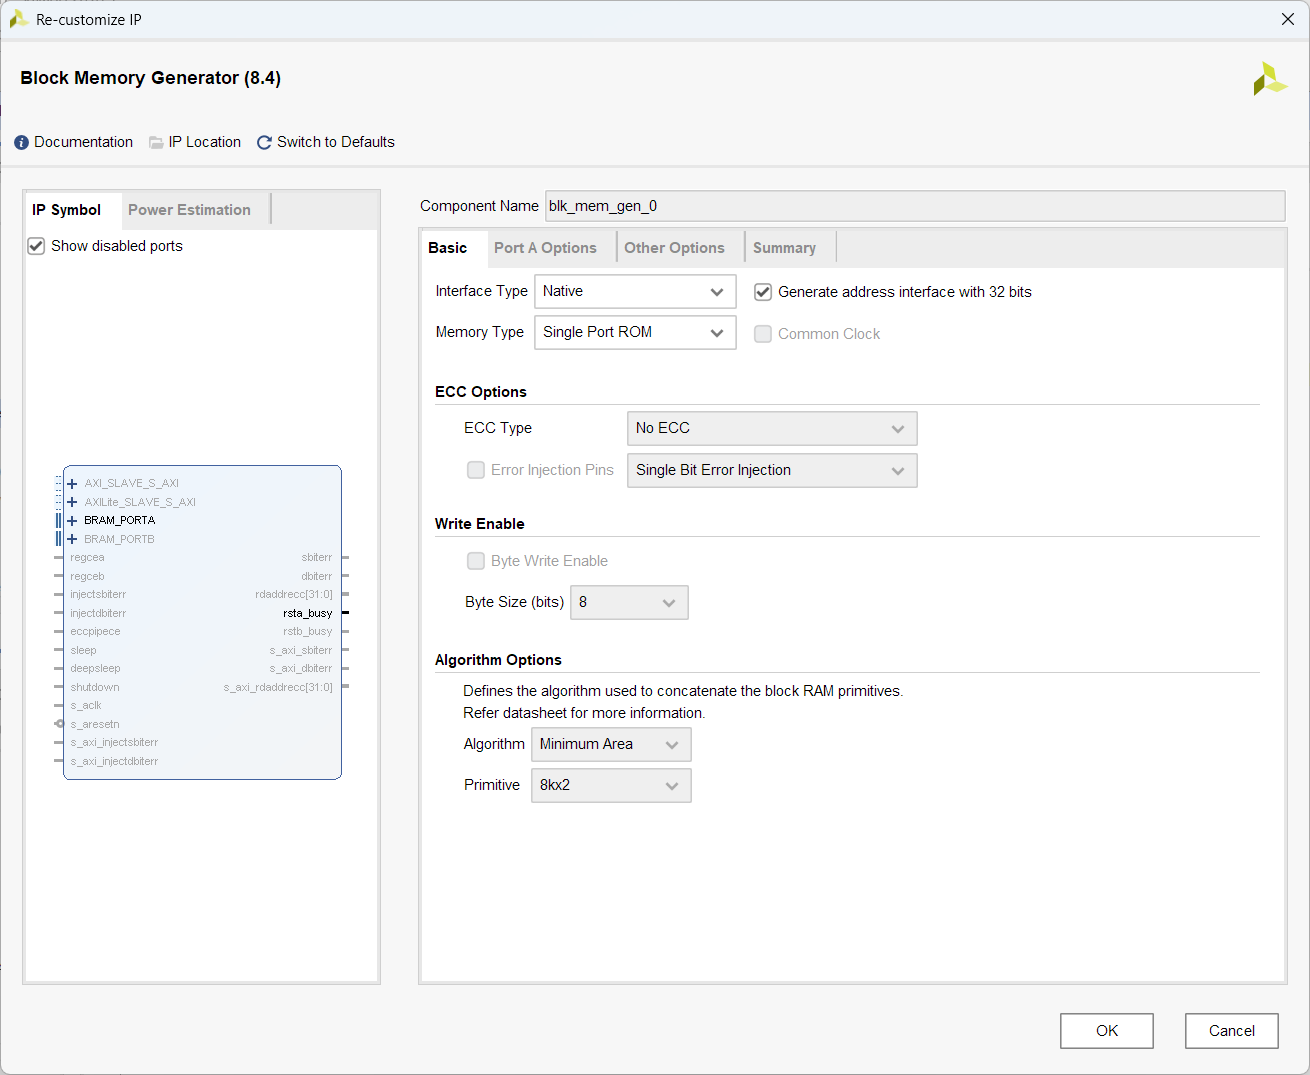
\includegraphics[width=0.7\textwidth]{image/pic1.png}
    \caption{存储器Basic界面}
	\label{fig:basic}
\end{figure}
\begin{figure}[H]
    \centering
    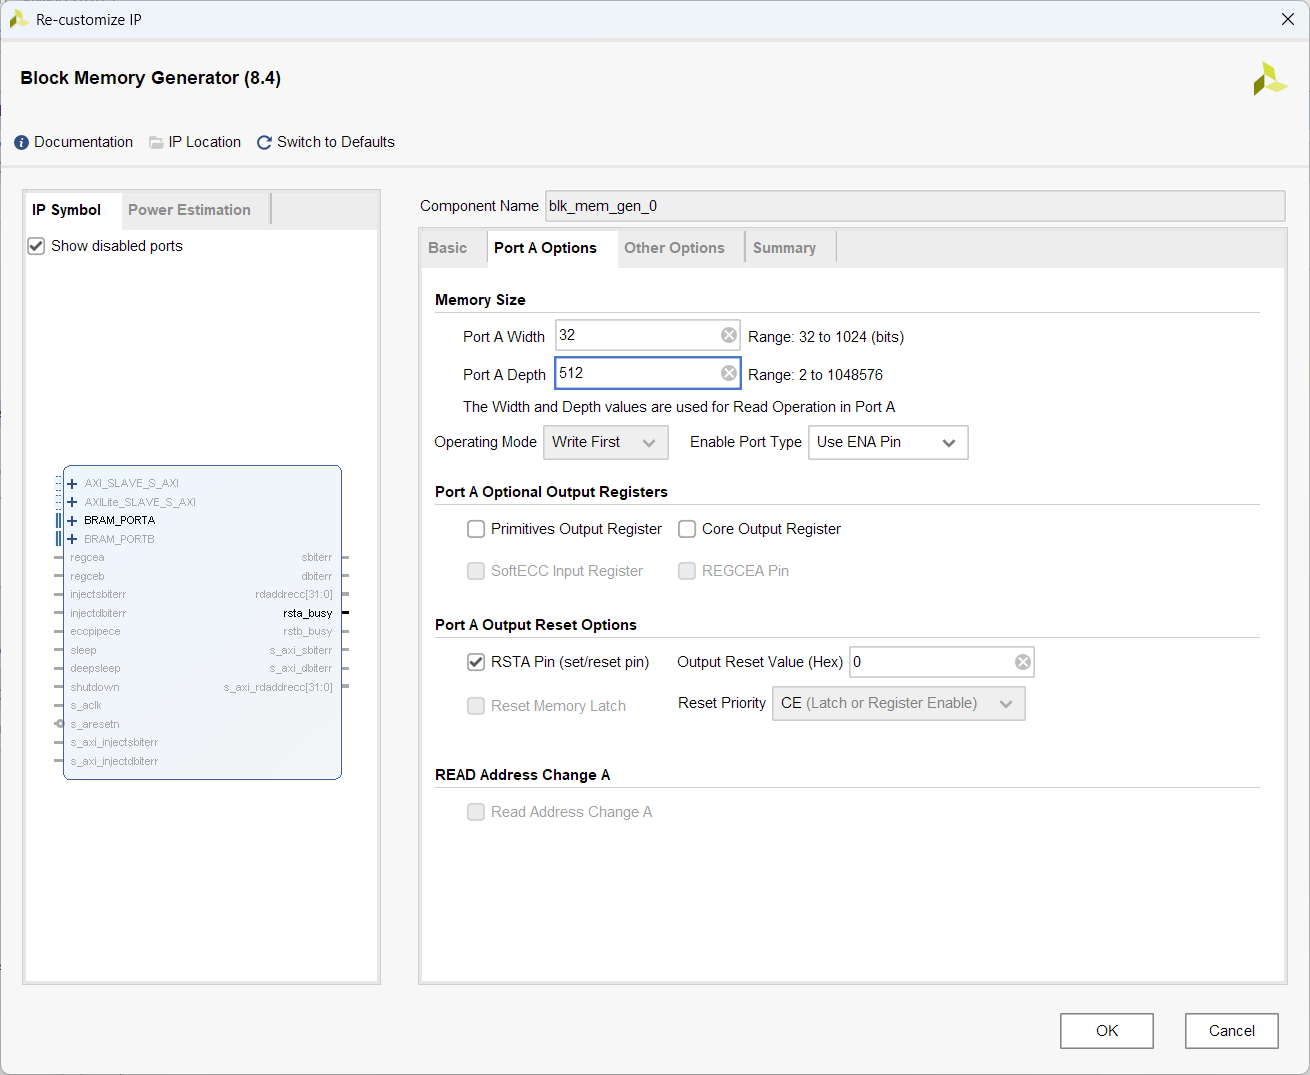
\includegraphics[width=0.7\textwidth]{image/pic2.png}
    \caption{存储器PartAOptions界面}
	\label{fig:partaoption}
\end{figure}
\begin{figure}[htbp]
    \centering
    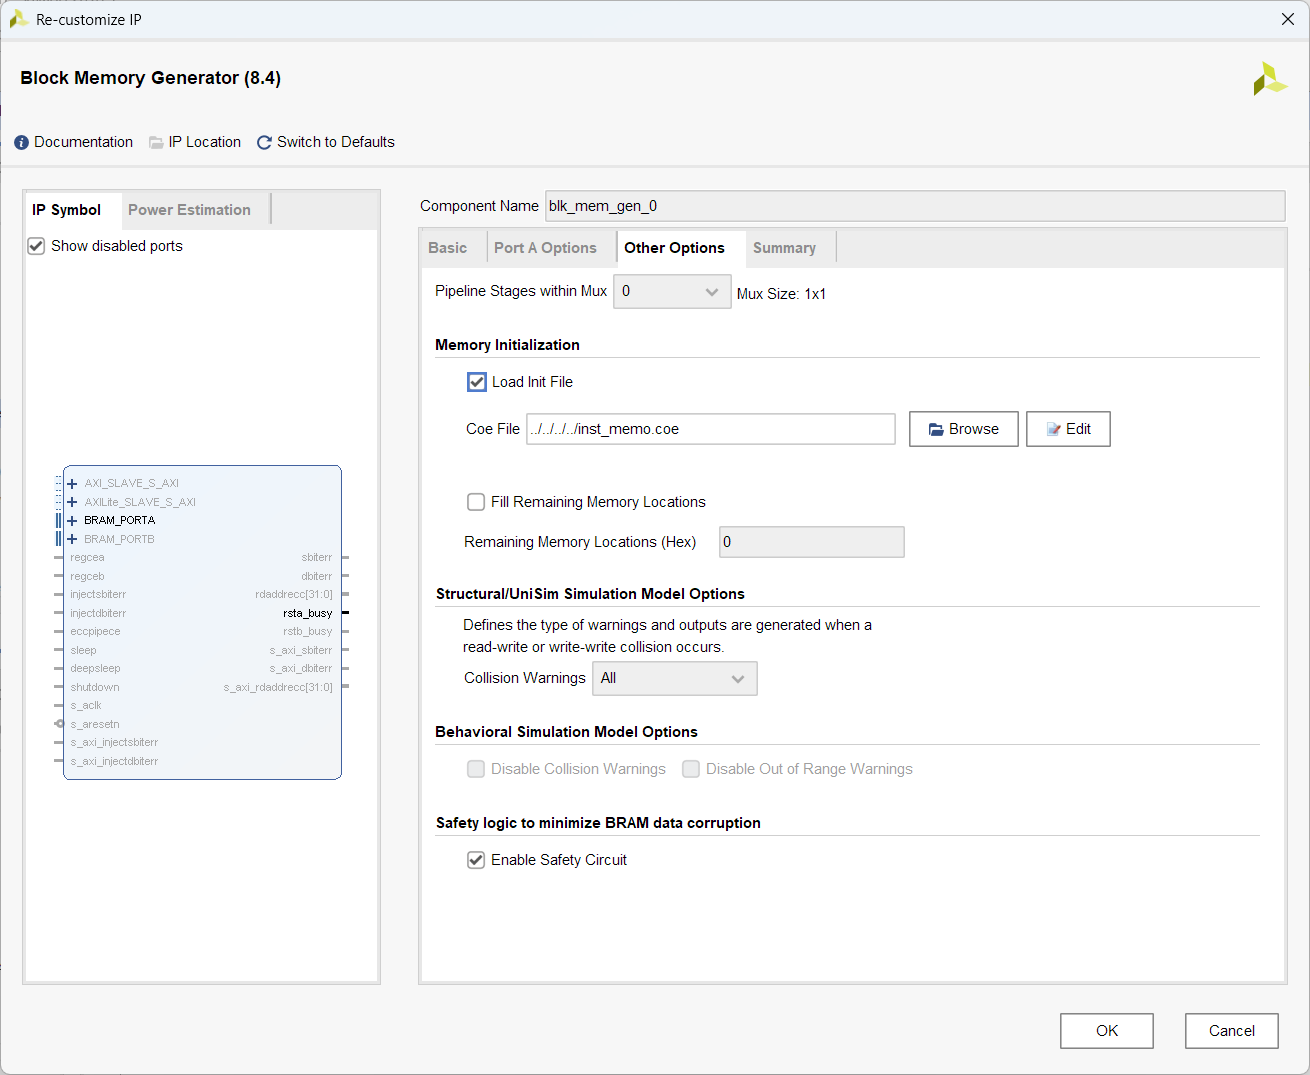
\includegraphics[width=0.7\textwidth]{image/pic3.png}
    \caption{存储器OtherOptions界面}
	\label{fig:otheroption}
\end{figure}
% \subsubsection{逻辑控制}

% \subsection{数据通路}\label{sub:dat}
% \subsubsection{功能描述}
% \subsubsection{接口定义}
% \subsubsection{逻辑控制}